

\tikzset{every picture/.style={line width=0.75pt}} %set default line width to 0.75pt        

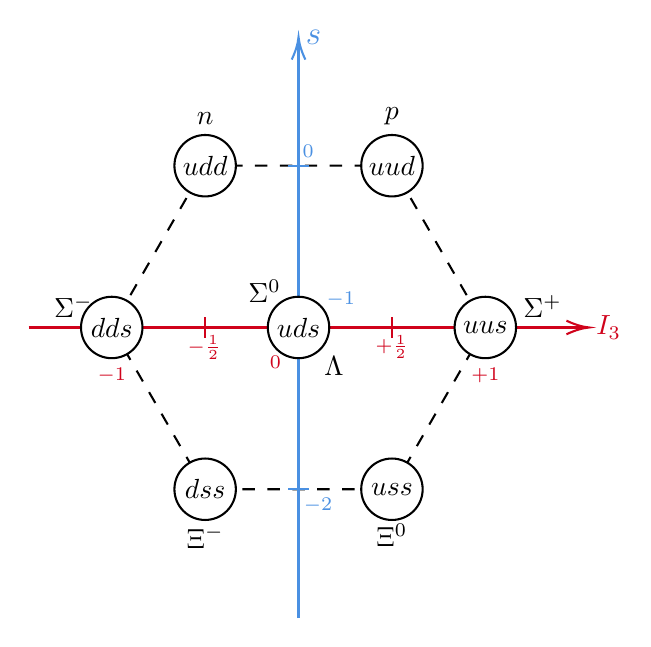
\begin{tikzpicture}[x=0.75pt,y=0.75pt,yscale=-1,xscale=1]
%uncomment if require: \path (0,314); %set diagram left start at 0, and has height of 314

%Shape: Regular Polygon [id:dp3461512214390913] 
\draw  [dash pattern={on 4.5pt off 4.5pt}] (232,162) -- (187,239.94) -- (97,239.94) -- (52,162) -- (97,84.06) -- (187,84.06) -- cycle ;
%Straight Lines [id:da7975119261953387] 
\draw [color={rgb, 255:red, 208; green, 2; blue, 27 }  ,draw opacity=1 ]   (12,162) -- (280,162) ;
\draw [shift={(282,162)}, rotate = 180] [color={rgb, 255:red, 208; green, 2; blue, 27 }  ,draw opacity=1 ][line width=0.75]    (10.93,-3.29) .. controls (6.95,-1.4) and (3.31,-0.3) .. (0,0) .. controls (3.31,0.3) and (6.95,1.4) .. (10.93,3.29)   ;
%Straight Lines [id:da49187250319695275] 
\draw [color={rgb, 255:red, 74; green, 144; blue, 226 }  ,draw opacity=1 ]   (142,302) -- (142,24) ;
\draw [shift={(142,22)}, rotate = 90] [color={rgb, 255:red, 74; green, 144; blue, 226 }  ,draw opacity=1 ][line width=0.75]    (10.93,-3.29) .. controls (6.95,-1.4) and (3.31,-0.3) .. (0,0) .. controls (3.31,0.3) and (6.95,1.4) .. (10.93,3.29)   ;
%Straight Lines [id:da04662903115423256] 
\draw [color={rgb, 255:red, 208; green, 2; blue, 27 }  ,draw opacity=1 ]   (97,157) -- (97,167) ;
%Straight Lines [id:da6078809997154113] 
\draw [color={rgb, 255:red, 208; green, 2; blue, 27 }  ,draw opacity=1 ]   (187,157) -- (187,167) ;
%Shape: Circle [id:dp2506066338504991] 
\draw  [fill={rgb, 255:red, 255; green, 255; blue, 255 }  ,fill opacity=1 ] (82.2,84.06) .. controls (82.2,75.88) and (88.83,69.26) .. (97,69.26) .. controls (105.17,69.26) and (111.8,75.88) .. (111.8,84.06) .. controls (111.8,92.23) and (105.17,98.86) .. (97,98.86) .. controls (88.83,98.86) and (82.2,92.23) .. (82.2,84.06) -- cycle ;
%Shape: Circle [id:dp49323091495562255] 
\draw  [fill={rgb, 255:red, 255; green, 255; blue, 255 }  ,fill opacity=1 ] (172.2,84.06) .. controls (172.2,75.88) and (178.83,69.26) .. (187,69.26) .. controls (195.17,69.26) and (201.8,75.88) .. (201.8,84.06) .. controls (201.8,92.23) and (195.17,98.86) .. (187,98.86) .. controls (178.83,98.86) and (172.2,92.23) .. (172.2,84.06) -- cycle ;
%Shape: Circle [id:dp2780130541001513] 
\draw  [fill={rgb, 255:red, 255; green, 255; blue, 255 }  ,fill opacity=1 ] (37.2,162) .. controls (37.2,153.83) and (43.83,147.2) .. (52,147.2) .. controls (60.17,147.2) and (66.8,153.83) .. (66.8,162) .. controls (66.8,170.17) and (60.17,176.8) .. (52,176.8) .. controls (43.83,176.8) and (37.2,170.17) .. (37.2,162) -- cycle ;
%Shape: Circle [id:dp22149042815123876] 
\draw  [fill={rgb, 255:red, 255; green, 255; blue, 255 }  ,fill opacity=1 ] (217.2,162) .. controls (217.2,153.83) and (223.83,147.2) .. (232,147.2) .. controls (240.17,147.2) and (246.8,153.83) .. (246.8,162) .. controls (246.8,170.17) and (240.17,176.8) .. (232,176.8) .. controls (223.83,176.8) and (217.2,170.17) .. (217.2,162) -- cycle ;
%Shape: Circle [id:dp2315285626329665] 
\draw  [fill={rgb, 255:red, 255; green, 255; blue, 255 }  ,fill opacity=1 ] (82.2,239.94) .. controls (82.2,231.77) and (88.83,225.14) .. (97,225.14) .. controls (105.17,225.14) and (111.8,231.77) .. (111.8,239.94) .. controls (111.8,248.12) and (105.17,254.74) .. (97,254.74) .. controls (88.83,254.74) and (82.2,248.12) .. (82.2,239.94) -- cycle ;
%Shape: Circle [id:dp3088315424845015] 
\draw  [fill={rgb, 255:red, 255; green, 255; blue, 255 }  ,fill opacity=1 ] (172.2,239.94) .. controls (172.2,231.77) and (178.83,225.14) .. (187,225.14) .. controls (195.17,225.14) and (201.8,231.77) .. (201.8,239.94) .. controls (201.8,248.12) and (195.17,254.74) .. (187,254.74) .. controls (178.83,254.74) and (172.2,248.12) .. (172.2,239.94) -- cycle ;
%Shape: Circle [id:dp27152267435822064] 
\draw  [fill={rgb, 255:red, 255; green, 255; blue, 255 }  ,fill opacity=1 ] (127.2,162) .. controls (127.2,153.83) and (133.83,147.2) .. (142,147.2) .. controls (150.17,147.2) and (156.8,153.83) .. (156.8,162) .. controls (156.8,170.17) and (150.17,176.8) .. (142,176.8) .. controls (133.83,176.8) and (127.2,170.17) .. (127.2,162) -- cycle ;
%Straight Lines [id:da5232366045305828] 
\draw [color={rgb, 255:red, 74; green, 144; blue, 226 }  ,draw opacity=1 ]   (137,84.1) -- (147,84.1) ;
%Straight Lines [id:da5088485977717139] 
\draw [color={rgb, 255:red, 74; green, 144; blue, 226 }  ,draw opacity=1 ]   (137,239.94) -- (147,239.94) ;

% Text Node
\draw (144,22) node [anchor=west] [inner sep=0.75pt]  [font=\large,color={rgb, 255:red, 74; green, 144; blue, 226 }  ,opacity=1 ]  {$s$};
% Text Node
\draw (284,162) node [anchor=west] [inner sep=0.75pt]  [color={rgb, 255:red, 208; green, 2; blue, 27 }  ,opacity=1 ]  {$I_{3}$};
% Text Node
\draw (142.5,72.65) node [anchor=north west][inner sep=0.75pt]  [font=\fontsize{0.71em}{0.85em}\selectfont,color={rgb, 255:red, 74; green, 144; blue, 226 }  ,opacity=1 ]  {$0$};
% Text Node
\draw (143.08,242.57) node [anchor=north west][inner sep=0.75pt]  [font=\fontsize{0.71em}{0.85em}\selectfont,color={rgb, 255:red, 74; green, 144; blue, 226 }  ,opacity=1 ]  {$-2$};
% Text Node
\draw (52,180.2) node [anchor=north] [inner sep=0.75pt]  [font=\fontsize{0.71em}{0.85em}\selectfont,color={rgb, 255:red, 208; green, 2; blue, 27 }  ,opacity=1 ]  {$-1$};
% Text Node
\draw (232,180.2) node [anchor=north] [inner sep=0.75pt]  [font=\fontsize{0.71em}{0.85em}\selectfont,color={rgb, 255:red, 208; green, 2; blue, 27 }  ,opacity=1 ]  {$+1$};
% Text Node
\draw (187.09,164.28) node [anchor=north] [inner sep=0.75pt]  [font=\fontsize{0.71em}{0.85em}\selectfont,color={rgb, 255:red, 208; green, 2; blue, 27 }  ,opacity=1 ]  {$+\frac{1}{2}$};
% Text Node
\draw (96.65,164.6) node [anchor=north] [inner sep=0.75pt]  [font=\fontsize{0.71em}{0.85em}\selectfont,color={rgb, 255:red, 208; green, 2; blue, 27 }  ,opacity=1 ]  {$-\frac{1}{2}$};
% Text Node
\draw (97,84.06) node    {$udd$};
% Text Node
\draw (187,84.06) node    {$uud$};
% Text Node
\draw (52,162) node    {$dds$};
% Text Node
\draw (142,162) node    {$uds$};
% Text Node
\draw (232,162) node    {$uus$};
% Text Node
\draw (97,239.94) node    {$dss$};
% Text Node
\draw (187,239.94) node    {$uss$};
% Text Node
\draw (97,65.86) node [anchor=south] [inner sep=0.75pt]    {$n$};
% Text Node
\draw (187,65.86) node [anchor=south] [inner sep=0.75pt]    {$p$};
% Text Node
\draw (97,256.14) node [anchor=north] [inner sep=0.75pt]    {$\Xi ^{-}$};
% Text Node
\draw (187,255.14) node [anchor=north] [inner sep=0.75pt]    {$\Xi ^{0}$};
% Text Node
\draw (44.38,158.82) node [anchor=south east] [inner sep=0.75pt]    {$\Sigma ^{-}$};
% Text Node
\draw (248.8,158.6) node [anchor=south west] [inner sep=0.75pt]    {$\Sigma ^{+}$};
% Text Node
\draw (135,151.6) node [anchor=south east] [inner sep=0.75pt]    {$\Sigma ^{0}$};
% Text Node
\draw (153,174.4) node [anchor=north west][inner sep=0.75pt]    {$\Lambda $};
% Text Node
\draw (135,174.4) node [anchor=north east] [inner sep=0.75pt]  [font=\fontsize{0.71em}{0.85em}\selectfont,color={rgb, 255:red, 208; green, 2; blue, 27 }  ,opacity=1 ]  {$0$};
% Text Node
\draw (154,153.6) node [anchor=south west] [inner sep=0.75pt]  [font=\fontsize{0.71em}{0.85em}\selectfont,color={rgb, 255:red, 74; green, 144; blue, 226 }  ,opacity=1 ]  {$-1$};


\end{tikzpicture}
